\documentclass[9pt,twocolumn,twoside]{pnas-new}
% add hyperref package
% \usepackage{hyperref}

% Use the lineno option to display guide line numbers if required.
% Note that the use of elements such as single-column equations
% may affect the guide line number alignment.
% new commands:

% species names
\newcommand{\cel}{\emph{C.~elegans}}
\newcommand{\dicty}{\emph{D.~discoideum}}
\newcommand{\ecol}{\emph{E.~coli}}

% gene names
\newcommand{\egl}{\emph{egl-9}}
\newcommand{\rhy}{\emph{rhy-1}}
\newcommand{\vhl}{\emph{vhl-1}}
\newcommand{\eglvhl}{\emph{egl-9;vhl-1}}
\newcommand{\eglhif}{\emph{egl-9;hif-1}}
\newcommand{\hif}{\emph{hif-1}}
\newcommand{\fog}{\emph{fog-2}}
\newcommand{\nhr}{\emph{nhr-57}}
\newcommand{\lam}{\emph{lam-3}}

% protein names
\newcommand{\eglp}{EGL-9}
\newcommand{\rhyp}{RHY-1}
\newcommand{\vhlp}{VHL-1}
\newcommand{\hifp}{HIF-1}
\newcommand{\fogp}{FOG-2}
\newcommand{\nhrp}{NHR-57}
\newcommand{\lamp}{LAM-3}

% DE genes numbers:
\newcommand{\egln}{1487}
\newcommand{\rhyn}{1816}
\newcommand{\vhln}{605}
\newcommand{\eglvhln}{1989}
\newcommand{\hifn}{481}
\newcommand{\eglhifn}{364}
\newcommand{\fogn}{1896}
\newcommand{\total}{3211}
\newcommand{\inall}{53}
\newcommand{\allup}{10}
\newcommand{\alldown}{13}

\newcommand{\egltargets}{}
\newcommand{\rhytargets}{}
\newcommand{\vhltargets}{25}
\newcommand{\hiftargets}{133}
\newcommand{\hifhydroxytargets}{}



\templatetype{pnasresearcharticle}[9pt,twocolumn,twoside,lineno] % Choose template
% {pnasresearcharticle} = Template for a two-column research article
% {pnasmathematics} = Template for a one-column mathematics article
% {pnasinvited} = Template for a PNAS invited submission

\title{Genetic Analysis of a Metazoan Pathway using Transcriptomic Phenotypes}

% Use letters for affiliations, numbers to show equal authorship (if applicable) and to indicate the corresponding author
\author[a,b, *]{David Angeles-Albores}
\author[a,b, *]{Carmie Puckett Robinson}
\author[a]{Brian Williams}
\author[a]{Igor Antoshechkin}
\author[a,b]{Paul W Sternberg}

\affil[a]{Department of Biology and Biological Engineering, Caltech, Pasadena, USA, 91125}
\affil[b]{Howard Hughes Medical Institute}
\affil[*]{These authors contributed equally to this manuscript}

% Please give the surname of the lead author for the running footer
\leadauthor{Angeles-Albores}

% Please add here a significance statement to explain the relevance of your work
\significancestatement{Measurements of global gene expression are often used as descriptive tools that identify genes that are downstream a perturbation. In theory, there is no reason why measurements of global transcriptomes could not be used as a quantitative phenotype for genetic analysis. Here, we show that transcriptomes can be used for epistasis analysis in a metazoan, and that transcriptomes afford far more information per experiment than classic genetic analysis. By using transcriptomes as quantitative phenotypes, we can accurately predict interactions between genes, while at the same time identifying genes common to a pathway.
When pathways branch, it is also possible to identify gene batteries that are associated with each end of the branch point. Finally, genes that would result in invisible visible phenotypes in an animal are not likely to be invisible at the transcriptome phenotype due to the exquisite granularity present in these structures, which represents an important advance towards studying small effect genes that make up the majority of animals' genetic repertoire.}

% Please include corresponding author, author contribution and author declaration information
\authorcontributions{DA, CPR and PWS wrote the manuscript. CPR performed all experiments. BW performed library preparation. IA performed sequencing. DA performed all analysis and blinded genetic reconstruction. DA, CPR and PWS designed the experiments.}
\authordeclaration{The authors declare no conflict of interest.}
% \equalauthors{\textsuperscript{1}A.O.(Author One) and A.T. (Author Two) contributed equally to this work (remove if not applicable).}
\correspondingauthor{\textsuperscript{2}To whom correspondence should be addressed. E-mail: pws@caltech.edu}

% Keywords are not mandatory, but authors are strongly encouraged to provide them. If provided, please include two to five keywords, separated by the pipe symbol, e.g:
\keywords{genetics $|$ RNA-seq $|$ \cel{} $|$ hypoxia $|$ transcriptomics}

\begin{abstract}
RNA-seq is a technology that is commonly used to identify genetic modules that are responsive to a perturbation. In theory, global gene expression could also be used as a phenotype, with all the implications that has for genetic analysis. To that end, we sequenced the transcriptome of four single mutants and two double mutants of the hypoxia pathway in \cel{}. We successfully analyzed the single mutants in a blinded fashion to predict the genetic relationships between the genes, and used the double mutants as a test of our predictions and to infer the directionality of the relationship.
We show that genes along a pathway tend to decorrelate as a result of alternative regulatory modes and crosstalk with other pathways; and that this decorrelation accurately reflects functional distance between genes. As a by-product of our analysis, we predict \hiftargets{} genes under the regulation of \hif{}, and \vhltargets{} genes under the regulation of \vhl{}. Transcriptomic perturbations suggest an important role of \hif{}-dependent response in chromatin remodelling in \cel{}. Interactive graphics for this paper can be found at \url{www.wormlabcaltech.github.io/mprsq}.\end{abstract}

\dates{This manuscript was compiled on \today}
\doi{\url{www.pnas.org/cgi/doi/10.1073/pnas.XXXXXXXXXX}}

\begin{document}


% Optional adjustment to line up main text (after abstract) of first page with line numbers, when using both lineno and twocolumn options.
% You should only change this length when you've finalised the article contents.
\verticaladjustment{-2pt}

\maketitle
\thispagestyle{firststyle}
\ifthenelse{\boolean{shortarticle}}{\ifthenelse{\boolean{singlecolumn}}{\abscontentformatted}{\abscontent}}{}

% If your first paragraph (i.e. with the \dropcap) contains a list environment (quote, quotation, theorem, definition, enumerate, itemize...), the line after the list may have some extra indentation. If this is the case, add \parshape=0 to the end of the list environment.
\dropcap{B}y definition, phenotypes are measurable traits that are related to genotypes via a formal mapping function. A requirement for a genetic relationship to exist is that two genes must act on the same phenotype. However, the converse, that two genes share a phenotype, does not imply that these genes interact. One way to prove genetic interaction is to measure epistasis in a double mutant. Epistasis refers to changes in a phenotype that are not additive and epistatic analysis remains an important cornerstone of genetics today~\cite{Phillips2008}.

Previous work in \emph{S. cerevisiae} and \dicty{} has shown that transcriptomes contain sufficient information to infer genetic relationships in a simple eukaryote~\cite{Hughes2000, VanDriessche2005}. This early work was performed using microarray technology, which suffered from drawbacks related to sensitivity. New technologies such as RNA-seq~\cite{Mortazavi2008} do not suffer from these drawbacks. Developments in the area of transcriptomics have also made important progress towards cheaper sequencing~\cite{Metzker2010}, better read alignment~\cite{Patro2014, Bray2015,Patro2015} and differential analysis~\cite{Pimentel2016,Trapnell2013}.
As a result, RNA-seq has been used to identify key regulatory modules involved in a variety of processes, including T-cell regulation~\cite{Singer2016,Shalek2013}, the \cel{} linker cell~\cite{Schwarz2012}, or planarian stem cell identification~\cite{VanWolfswinkel2014,Scimone2014}. However, even in these novel applications, transcriptomes largely serve a descriptive role, and are important for hypothesis generation and target acquisition as opposed to hypothesis testing and model creation.

To investigate the ability of transcriptomes to serve as quantitative phenotypes, we selected mutants in the \cel{} hypoxia pathway for transcriptome sequencing. The hypoxia pathway is a conserved pathway that is found in all metazoans~\cite{Semenza2012}. It plays an important role in oxygen and iron homeostasis and in the immune response among others~\cite{Nizet2009,Ackerman2012}, and it is believed to play an important role in cancer appearance and progression, making it an attractive therapeutic target for disease~\cite{Semenza2003}.
 In \cel{} and other systems, \hifp{} is constitutively degraded by a futile cycle that involves hydroxylation by the EGLN1 ortholog \eglp{}, followed by ubiquitination by the von Hippel-Lindau Suppressor 1, \vhlp{}~\cite{Bishop2004,Shao2009,Tanimoto2000,Jaakkola2001}. Inhibition of hydroxylation leads to accumulation of activated \hifp{}~\cite{Bishop2004}. Among the known targets of \hifp{} activation are \rhy{} and \egl{}. Increased \rhyp{} levels lead to activation of \eglp{} protein by inhibition of CYSL-1 which is an inhibitor of \eglp{}~\cite{Shen2006,Ma2012}.

Here, we show that transcriptomes contain extremely strong, robust signals that can be used to infer relationships between genes in complex metazoans by reconstructing a the hypoxia pathway in \cel{} using RNA-seq in a blinded manner. Our goal is not to generate a high-quality database of hypoxia-related genes, but rather to perform a quantitative genetic analysis analogous to classical genetics. Using this experimental setup, we show that various techniques, including pairwise comparisons, clustering or \emph{in silico} qPCR can be used to generate a testable model of genetic interactions. A complete, interactive version of the analysis is also available at \url{www.wormlabcaltech.github.io/mprsq}.

\section*{Results}
\subsection{Clustering visualizes epistatic relationships between genes}
\label{sub:Clustering}

As a first step in our analysis, we analyzed our data using a generalized linear model with a genotype term (see~\ref{methods}) on logarithm-transformed counts. Genes that are significantly altered between wild-type and a given mutant have a genotype coefficient that is statistically significantly different from 0. We refer to these coefficients through the greek letter $\beta$. These coefficients are not identical to the average log-fold change per gene, although they are loosely related to this quantity. In general, larger $\beta$ magnitudes correspond to larger perturbations. These coefficients can be used to study the RNA-seq data in question.

Clustering is a well-known technique in bioinformatics that is used to identify relationships between data~\cite{Yeung2003}. We wanted to make sure that clustering by differential expression yielded genetically relevant information. \hif{} is known to be inhibited by a pathway involving \egl{}, \vhl{} and \rhy{}. \egl{}; \hif{} mutants exhibit suppression of the \emph{egl} phenotype. Given this information, \hif{} should cluster near the \egl{}; \hif{} double mutant.
Indeed, when blind, unsupervised clustering was performed on the data, three clusters emerged. \hif{} and \egl{};\hif{} clustered together, indicating suppression of the \egl{} phenotype; whereas \egl{}, \egl{};\vhl{}, \vhl{} and \rhy{} all clustered separately. Finally, our negative control \fog{} was in its own cluster (see Fig.~\ref{fig:dendrogram}). Thus, we conclude that expression data contains enough signal to cluster genes in a meaningful manner.

% dendrogram
\begin{figure}%[tbhp]
\centering
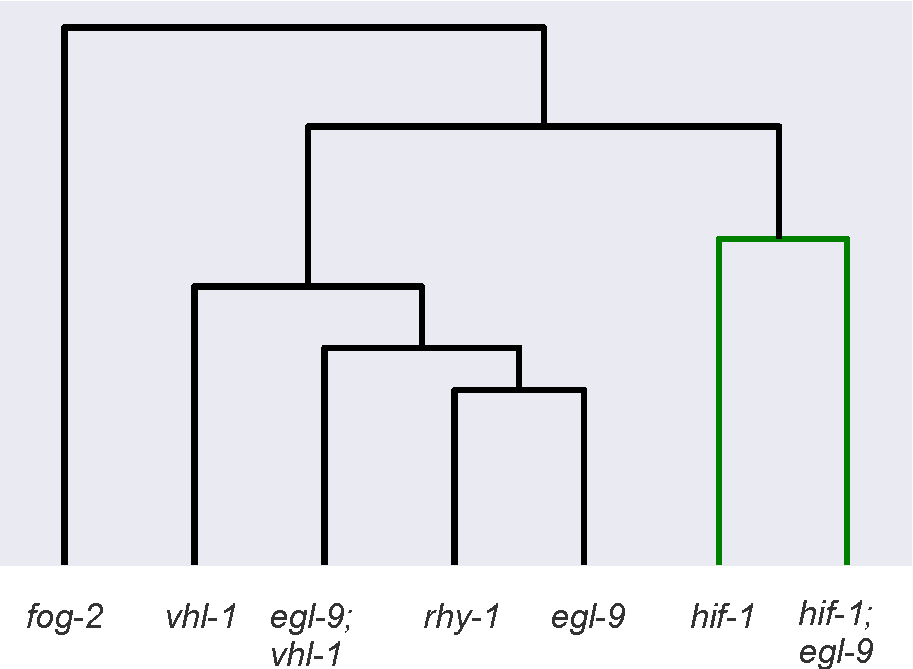
\includegraphics[width=\linewidth]{figs/dendrogram.pdf}
\caption{Blind unsupervised clustering of various \cel{} mutants. Genes cluster in a manner that is biologically intuitive. Genes that inhibit \hif{} (i.e, \egl{}, \vhl{}, and \rhy{}) cluster far from \hif{}. \hif{} clusters with the suppressed \egl{}; \hif{} double mutant. A control gene, \fog{}, clusters farthest away.}
\label{fig:dendrogram}
\end{figure}

\subsection{Transcriptomic correlations can predict genetic regulation}
\label{sub:Transcriptomic genetic analyses}

% TODO: Add SI link at end of paragraph.
Theoretically, two genes that share linear positive regulation should be positively correlated in their overlapping transcriptomes, whereas two genes that share linear negative regulation should be negatively correlated in their transcriptomes. Formally, if we consider that a gene \emph{A} has a transcriptome \emph{\{A\}} associated with it, and if we consider a second gene \emph{B} with an associated transcriptome \emph{\{B\}} that is activated by \emph{A} (that is, $B \in \{A\}$, such that $\{B\} \subset \{A\}$), then it follows that genetic knockout of \emph{A} or \emph{B} should both lead to the same perturbation of the transcriptome \emph{\{B\}}. Conversely, it follows that if two mutants have overlapping transcriptomes, and if these transcriptomes have a strong positive association, it is likely that these two genes share a positive regulatory association. In other words, transcriptomic correlation is a good predictor of genetic regulation. For a formal introduction to the genetic logic, see S.I..

Although transcriptomic correlations could theoretically be used for the purposes of identifying genetic regulation, noise from measuring 20,000 genes in multiple different genotypes can cause serious interference with any inferences. Additionally, genes sometimes experience multiple modes of regulation, including positive and negative regulation, from the same gene or pathway. Because we are measuring the system at steady state, both modes of regulation will be measured simultaneously. If a positive and a negative signal are both present in a transcriptome, running a naive regression may result in a value close to zero.
Therefore, we took steps to mitigate noise emanating from frequent outliers. As a first mitigation attempt, we rank-tranformed the $\beta$ coefficients for each mutant. This has the effect of mitigating outliers by resetting the difference between adjacent coefficients to unity. Secondly, we performed robust Bayesian regressions using a Student T distribution as a prior. A Student T distribution decays less quickly than a normal distribution, which causes the model to consider outliers to be less informative than traditional frequentist regressions which effectively use a normal prior.

% genetic correlations
\begin{figure}%[tbhp]
\centering
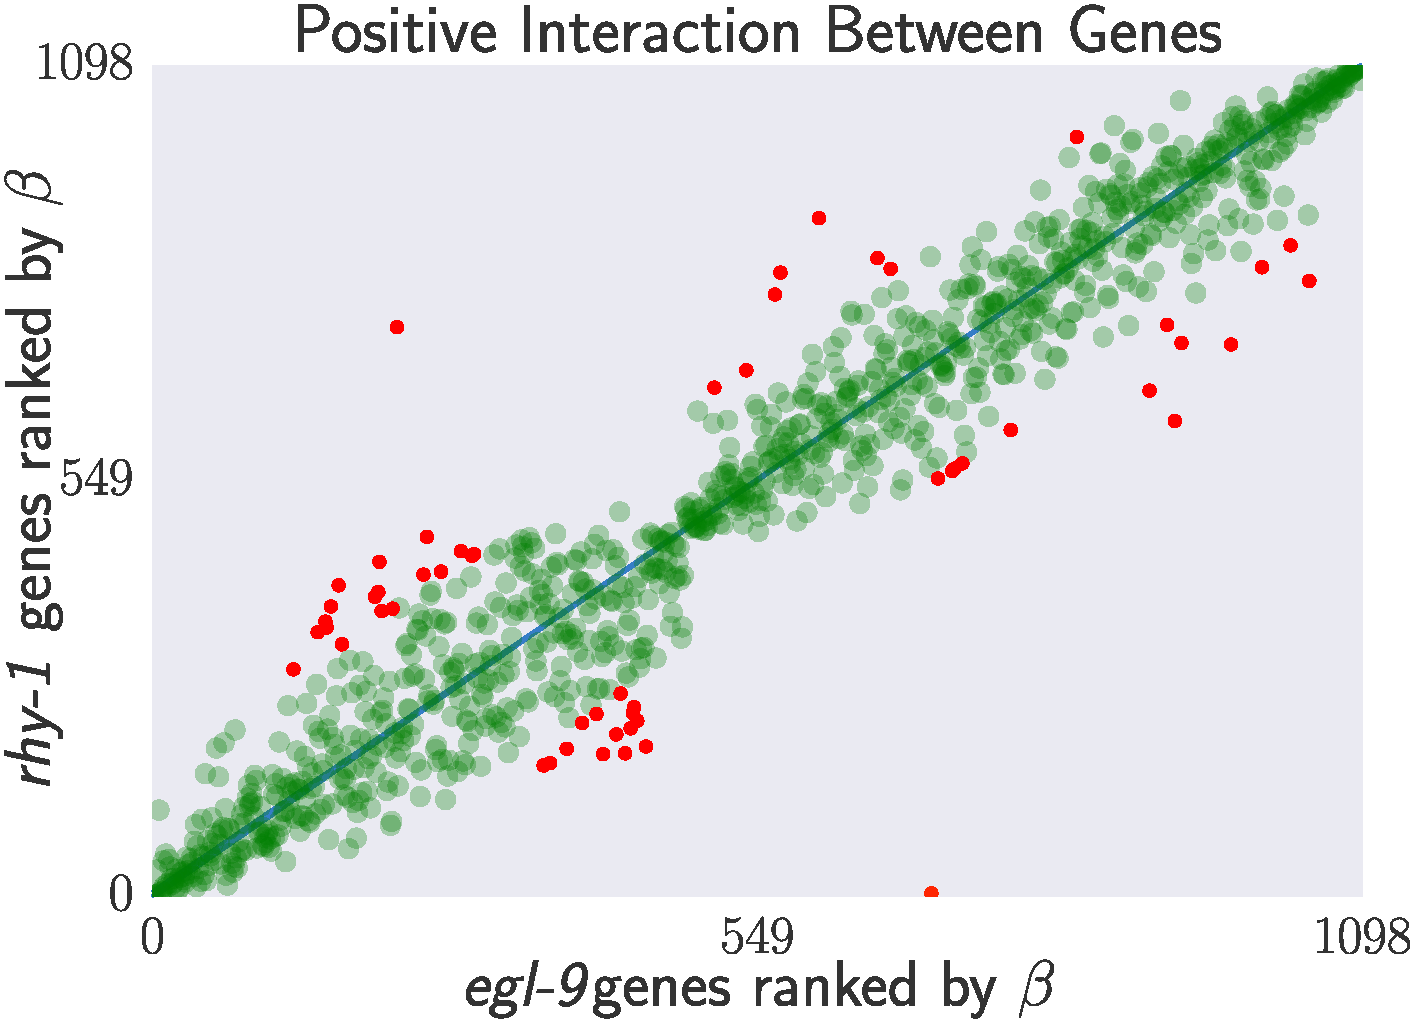
\includegraphics[width=0.85\linewidth]{figs/correlative_genetics.pdf}
\caption{\textbf{Top} Schematic Diagram showing that genes that interact positively should have a positive transcriptomic correlation, whereas genes that interact negatively should have a negative correlation. Single genes are referred to by their names (A, B), and the transcriptome associated only with gene X is referred to as \{X\}. We use superscripts to denote expression level. In this case, 0 = no expression (knockout); 1 = WT level; 2 = Greater than WT level.\ \textbf{Bottom} Empirical demonstration that transcriptomes between two interacting genes can be extremely well correlated when genes are ranked by expression changes relative to a wild-type.}
\label{fig:genetic_interactions}
\end{figure}

% TODO: Check if egl was in fact first identified as a hif target
% TODO: SI links
Having mitigated the effect of outliers, we saw that for certain gene pairs, their transcriptomes correlated very well when genes were ranked by their expression changes (see Fig.~\ref{fig:genetic_interactions}). Having confirmed that we can extract strong signals from these transcriptomes, we proceeded to generate all pairwise correlations between transcriptomes and we weighted the correlations by the number of genes that participated in the correlation (that were not outliers) divided by the total number of genes detected in all samples.
The regression slopes recapitulated a network with three `modules': A control module, a responder module and an uncorrelated module (see Fig.~\ref{fig:heatmap}). We were able to identify a strong positive interaction between \egl{} and \rhy{}. Part of the reason for this lies in the fact that the transcriptomes for these genes consisted of \egln{} and \rhyn{} significantly altered genes respectively and the overlap between both genes was quite extensive.
On the other hand, none of the primary correlations between \hif{} and its controlling genes are negative. We suspect that this is a result of the profound control that \hif{} exerts on \egl{} and \rhy{}. See SI A and B for an exhaustive analysis of the expected and observed correlation between each gene pair in this circuit respectively.
% heatmap
\begin{figure}[tbhp]
\centering
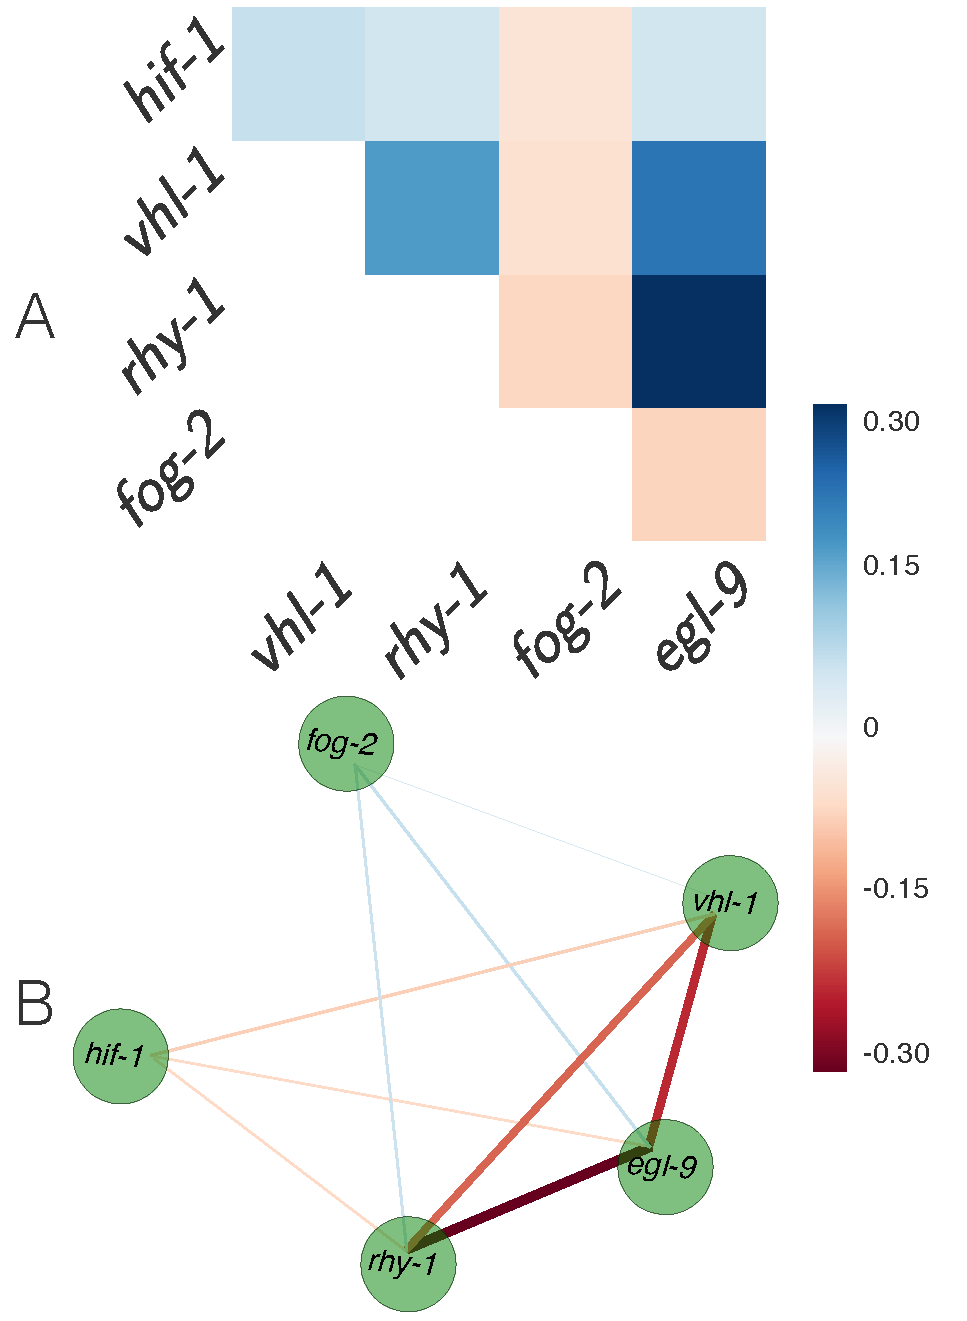
\includegraphics[width=0.85\linewidth]{figs/bayesian_heat_map.pdf}
\caption{\textbf{Top}: Heatmap showing pairwise regression values between all single mutants. \textbf{Bottom}: Correlation network drawn from the diagram. Edge width is directly proportional to the regression value.}
\label{fig:heatmap}
\end{figure}

Previous work in the hypoxia pathway suggests that this pathway may have feedback loops. Using the same genetic formalism as above, we realized that interactomes due to the fine-grained nature of the data can identify two regulatory interactions if they are of opposite sign. Consider a system in which an arbitrary gene A activates a gene B, which in turn blocks a gene C. Each gene X has a specific transcriptome \emph{\{X\}}.Under this system, B and C should have transcriptomes that are negatively correlated. If C activates A, however, then knocking out B should augment expression of C, which should in turn increase expression of A.
However, knocking out C should lead to less A, which in turn will lead to less B. Under this thought experiment, suppose that we know the specific transcriptomes associated with A, B and C:\@\emph{\{A\}}, \emph{\{B\}}, \emph{\{C\}}. Then it must be the case that the genetic knockout of B must have a perturbed transcriptomes $\{A^2\}, \{B^0\}, \{C^2\}$-in other words, knocking out B increases the levels of A, which leads to an overexpression perturbation of the specific transcriptome associated with A, and so forth. On the other hand, knocking out C must lead to the perturbed transcriptomes $\{A^0\}, \{B^0\}, \{C^0\}$.
Now, if we were able to correlate each specific transcriptome between correlations, we would find that the specific transcriptomes associated with A and C are anti-correlated; whereas the specific transcriptome associated with B is correlated between both genotypes. This should lead to a characteristic \emph{X} pattern in the ranked data. Although in this particular example the cross is due to feedback loops, it is important to point out that there are other patterns that could generate crosses.
% correlative genetics again
\begin{figure}[tbhp]
\centering
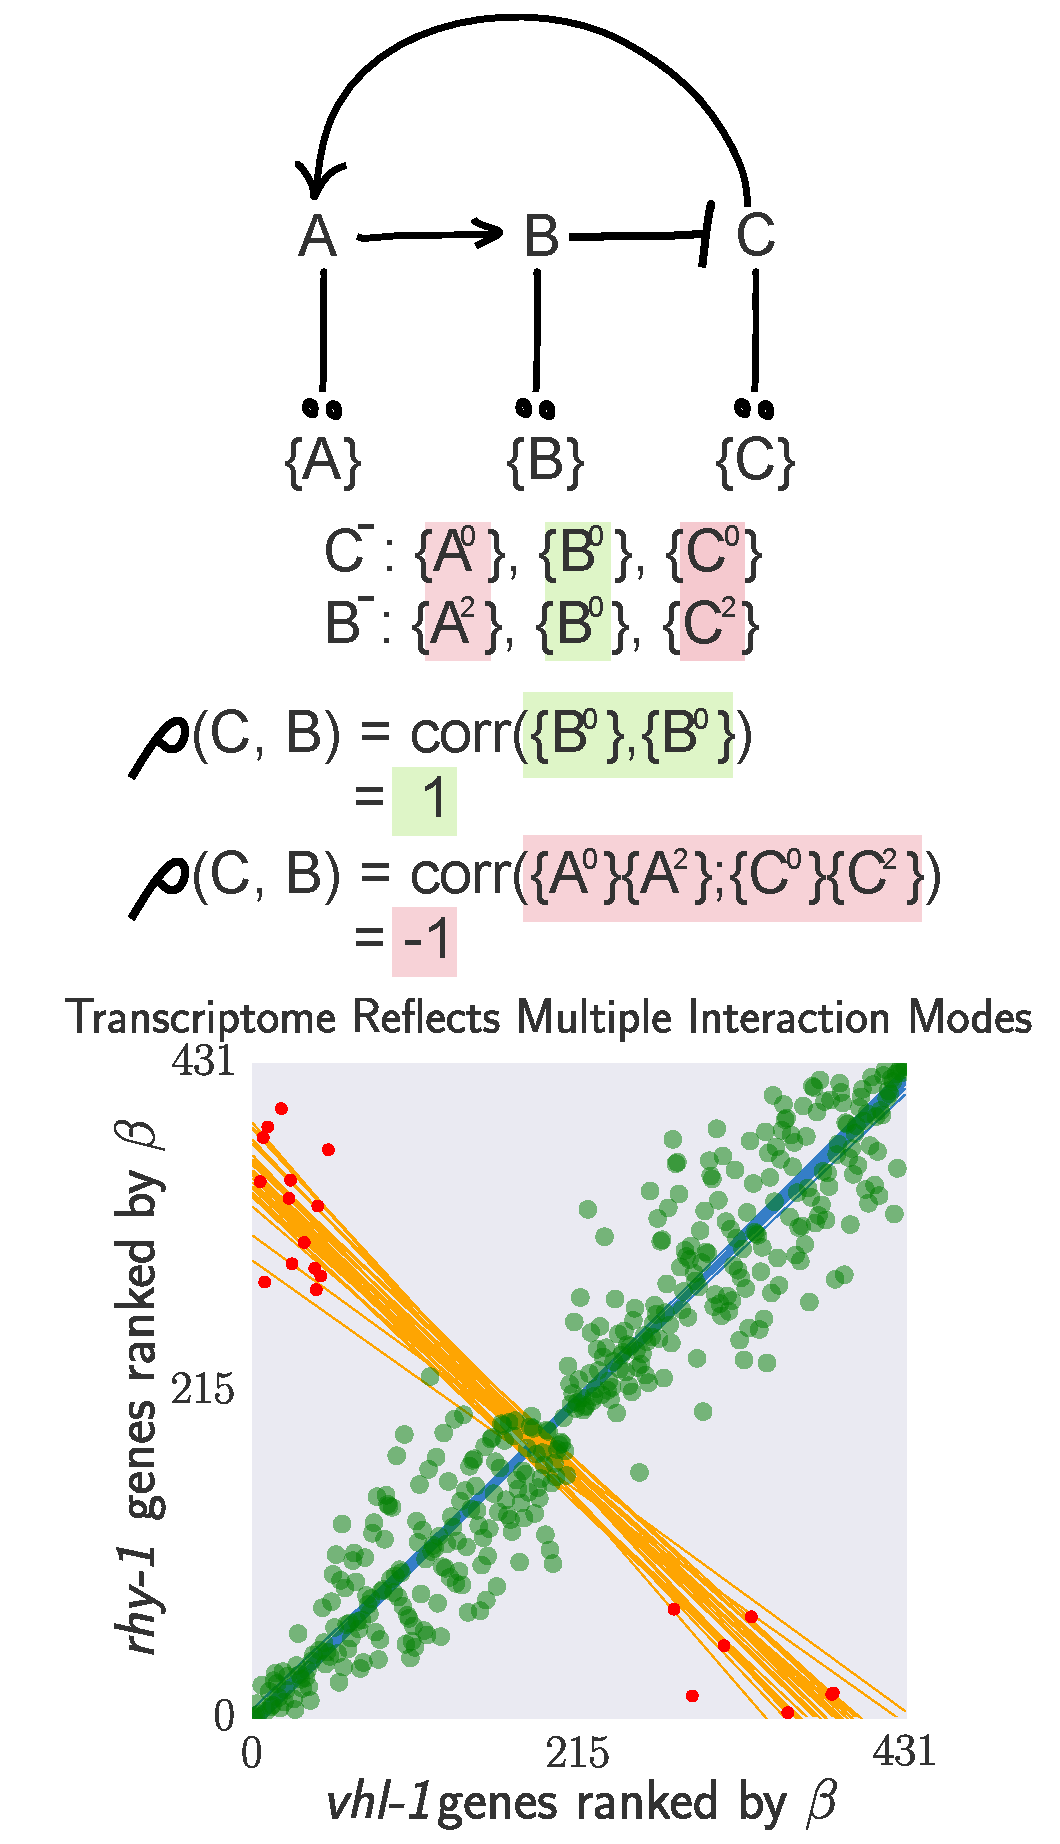
\includegraphics[width=\linewidth]{figs/correlative_genetics2.pdf}
\caption{\textbf{Top}: A feedback loop can generate transcriptomes that are both correlated and anti-correlated. \textbf{Bottom}: \hif{} transcriptome correlated to the \rhy{} transcriptome. Green large points are inliers to the first regression. Red small points are outliers to the first regression. Only the red small points were used for the secondary regression. Blue lines are representative samples of the primary bootstrapped regression lines. Orange lines are representative samples of the secondary bootstrapped regression lines.}
\label{fig:xpattern}
\end{figure}

% TODO SI link
We investigated whether any pairwise comparisons between our single mutants generated this cross pattern. Indeed, we found that comparing \hif{} with \rhy{}, and \hif{} with \egl{} yielded negative correlations, as did \rhy{} and \vhl{}. While the number of genes that lead these negative correlations is not significant as assessed by a hypergeometric test, these outliers are expected for this circuit (see SI). Statistical information should be integrated holistically with genetic models to assess whether outliers are meaningful or not. Since \hif{} was off in the conditions under which we performed our experiment, measurement of the \hif{} transcriptome is difficult and we suspect the small number of outliers is the result of this low resolution.


\subsection{\emph{in silico} qPCR reveals extensive feedback in the hypoxia pathway}
\label{sub:qPCR}
We realized that our dataset enabled us to perform a sort of \emph{in silico} qPCR.\@ To verify the quality of our data and the veracity of \emph{in silico} qPCR, we first queried the changes in expression of \nhr{}. This particular reporter has been shown to be under direct control of \hif{}. Thus, we expected that this gene should go up in \egl{}, \rhy{} and \vhl{}, and it should be unchanged in \hif{}. The epistasis test, using the double \egl{};\hif{} double mutant should result in no change; whereas the \egl{};\vhl{} double mutant should have a similar change to the \vhl{} and the \egl{} mutants. In fact, our datasets reflected these known interactions, showing that the RNA-seq measurements can be used in a semi-quantitative fashion to perform inferences on genetic regulation.
% in silico qPCR
\begin{figure}[tbhp]
\centering
\includegraphics[width=\linewidth]{figs/qpcr.pdf}
\caption{\textbf{Top}: \emph{In silico} qPCR results. \nhr{} is an expression reporter that has been used previously to identify \hif{} regulators~\cite{Shen2006,Shao2009}. The \nhr{} mRNA levels replicate what is observed in the literature and serves as a quality control for our dataset. \lam{} is a negative control that should not be involved in this pathway. Changes in the hypoxia pathway suggest that \hif{} activates \rhy{}, and possibly \egl{}, when it is not hydroxylated. \hif{} also appears to autoactivate in a hydroxylation-dependent manner.}
\label{fig:qpcr}
\end{figure}

% TODO: Verify the next paragraph is true.
Next, we decided to perform \emph{in silico} qPCR of every gene under scrutiny to get a clearer idea of the relationships between them (see Fig.~\ref{fig:qpcr}). We found that \rhy{} transcription levels, and to a lesser extent \egl{} levels were increased by mutations in \egl{}, \rhy{} and \vhl{}. This suggests that \hif{} is a positive regulator of \rhy{}.
Given that \rhy{} post-translationally controls \egl{}~\cite{Ma2012}, it is unlikely that the increase in \egl{} is driven by the increase in \rhy{} levels. Therefore, our experiment also suggests that \hif{} is a positive regulator of \egl{}. On the other hand, we also discovered that mutation of \hif{} increased levels of \rhy{}. This suggests that \hif{} is also a negative regulator of \rhy{}. One potential mechanism through which \hif{} could be both a positive and a negative regulator would be for hydroxylation of \hif{} to change its activity. Under this mechanism, loss of \hif{} hydroxylation leads to activation of \rhy{} and \egl{} as a homeostatic mechanism, whereas excessive hydroxylation causes inhibition of these genes.

% TODO: Review the hif mRNA stuff and make sure it's good.
Whereas loss of hydroxylation seems to lead to overexpression of \rhy{} and \egl{}, there is no change in \hif{} levels. The only change in expression level of this gene occurs in the \hif{} mutant\footnote{We cannot discard the possibility that this decrease in mRNA levels is not due to NMD or some other decay mechanism, but we consider such a large change unlikely}. Therefore, we postulate that \hif{} positively autoregulates itself only in its non-hydroxylated state. We propose that increasing \hifp{} levels through inactivation of \eglp{} does not increase \hif{} mRNA levels because \hif{} is already autoactivating at its maximum rate under normoxia, which should happen if \hifp{} has a very strong tendency to autoactivate.

Performing the \emph{in silico} experiment with the \egl{};\vhl{} double mutant shows a similar increase in activity of the two genes in question.
This provides confirmatory evidence that \hif{} up-regulates \egl{}, but also suggests that \egl{} and \vhl{} are epistatic to one another. Such epistasis can only occur in one of two ways: Either the genes are acting linearly, or they are acting in AND gated fashion, with both genes required to mediate an effect. Similarly, the \egl{};\hif{} double mutant exhibits the same expression profile as \hif{}, which means \egl{} is an inhibitor of \hif{}.

% decorrelation
\begin{figure}[tbhp]
\centering
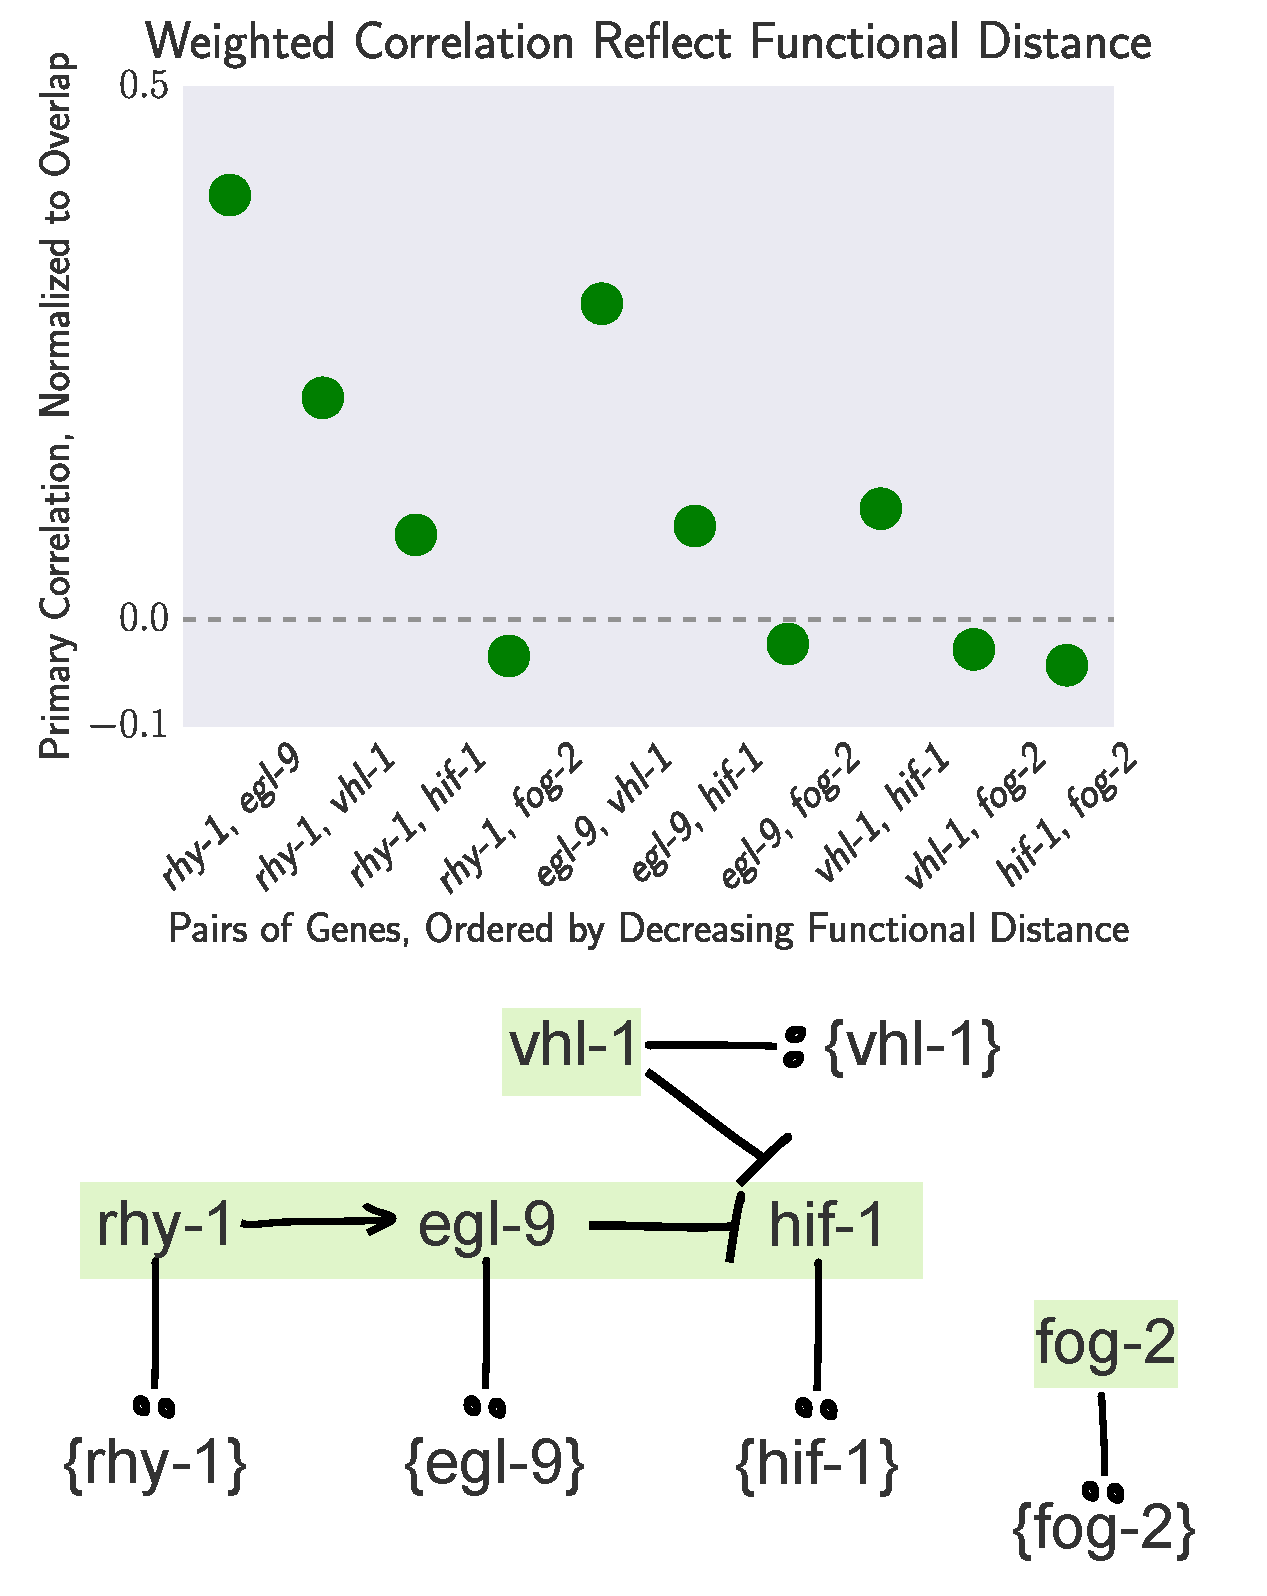
\includegraphics[width=\linewidth]{figs/functional_distance.pdf}
\caption{Top: Pairwise weighted correlations between transcriptomes can be used to infer functional distance between interacting genetic partners. Pairwise correlations are ordered by increasing network distance between genes. Correlations were weighted by the fraction of genes that overlapped between the two genes being compared. Notice that correlations involving the \fog{} negative control are very near zero. Error bars represent standard deviation of the weighted correlation. Bottom: Simplified schematic of the hypoxia pathway shown to illustrate functional distance between genes in the pathway.}
\label{fig:decorrelation}
\end{figure}

In summary, the \emph{in silico} qPCR results suggest that \egl{} and \vhl{} act in concert to inhibit \hif{}. Likewise, these results taken together with the transcriptome-wide cross-patterns that emerge from pairwise comparisons between genes in the hypoxia pathway suggest that there are positive and negative feedback loops feeding into \rhy{} and possibly \egl{}. These feedack loops explain why \hif{} is positively transcriptomically correlated with \egl{}.

\subsection{Epistasis effects can be detected and quantified.}
\label{sub:Epistasis}
To discover whether there is evidence of \egl{} and \vhl{} acting independently of each other in our dataset, we identified the genes that were shared between each single mutant and the double mutant \egl{};\vhl{}. If two genes act, for example, in a linear manner, then the double mutant should exhibit an identical phenotype to each single mutant. To test such a relationship, we can plot the change in $\beta$ coefficients between a single and double mutant versus the $\beta$ coefficient in the respective single mutant and fitting a weighted linear regression to measure the slope of best fit. Genes that act in a linear pathway should yield lines with a slope of 0. Genes that have some additive flavor should have slopes greater than 0. Suppression, a hallmark of inhibition, should yield a slope less than 0.

We observe that the \egl{};\vhl{} mutant has an identical phenotype to the \egl{} single mutant (slope = 0; see Fig.~\ref{tab:double_mutant_comparison}). On the other hand, \vhl{} has a positive slope, indicating that \egl{} is additive to \vhl{}. Such partial additivity can be explained if \egl{} is inhibiting \hif{} in a \vhl{}-dependent as well as a \vhl{}-independent manner~\cite{Shao2009}.
% double mutant analysis
\begin{table}%[tbhp]
\centering
\caption{Response Modeling of Double Mutants to Single Mutants}
\begin{tabular}{llrrr}
Double Mutant & Single Mutant & $\Delta$ & SEM & p-value\\
\midrule
1. \egl{};\vhl{} & \egl{} & $0.0$ & $0.01$ & $0.81$\\
2. \egl{};\vhl{} & \vhl{} & $0.28$ & $0.033$ & $10^{-15}$\\
3. \egl{};\hif{} & \egl{} & $-0.85$ & $0.074$ & $10^{-13}$\\
4. \egl{};\hif{} & \hif{} & $-0.18$ & $0.10$ & $0.097$\\
\bottomrule
\end{tabular}

\addtabletext{Table showing changes between single and double mutants. $\Delta$ is the result of a weighted-linear regression (WLS) between $\beta_\mathrm{single}$ and $\beta_\mathrm{double} - \beta_\mathrm{single}$. $\Delta$ > 0 represents a more severe phenotype than the single mutant. $\Delta$ < 0 represents a suppressed phenotype relative to the single mutant. $\Delta$ = 0 is expected for linear pathways or genes that are acting in linear or AND-gated fashion. $\Delta > 0$ is expected for genes that are acting additively on a pathway. WLS were performed only on genes that were significantly altered in both single mutants and the double mutant. $1+\Delta$ is a very close approximation to the line of best fit between single mutant and double mutant.}
\label{tab:double_mutant_comparison}
\end{table}

On the other hand, comparison of the \egl{};\hif{} double mutant showed suppression of the \egl{} transcriptomic phenotype. This suppression is expressed in various ways. First, the double mutant shows less statistically significantly differentially expressed genes than either single mutant. Secondly, these genes change less on average than they do in \egl{}, but the average change is the same as \hif{}.

\subsection{Transcriptomic decorrelation can be used to infer functional distance}
\label{sub:decorrelation}
We were interested in figuring out whether RNA-seq could be used to identify functional interactions within a genetic pathway. Although there is no \emph{a priori} reason why global gene expression should reflect functional interactions, the strength of the unweighted correlations between genes in the hypoxia pathway made us wonder how much information can be extracted from this dataset.

We investigated the possibility that transcriptomic signals might contain relevant information about the degrees of separation by weighting the robust bayesian regression of each pairwise analysis by $N_\mathrm{Overlap}/N_{\mathrm{detected}}$. We then plotted the weighted correlation of each gene pair, ordered by increasing functional distance (see Fig.~\ref{fig:decorrelation}). In every case, we see that the weighted correlation decreases monotonically due mainly, but not exclusively, to decreasing $N_\mathrm{Overlap}$.
We believe that this result is not due to random noise or insufficiently deep sequencing. Instead, we propose a framework in which every gene is regulated by multiple different molecular species. Even in unbranched pathways, this would induce progressive decorrelation between genes.

\subsection{Identification of novel targets and biological processes in the hypoxia response}
\label{sub:new_biology}
% TODO: Add SI folder information
So far, our analysis has focused mainly on extracting genetic relationships between the set of mutants we sequenced. It has not escaped our attention that our dataset also provides us with a unique view of the \hif{}-dependent response in \cel{}. In total, we identified \total{} differentially expressed genes that are altered in any of the hypoxia pathway mutants. Of these \total{} genes, \inall{} genes were differentially expressed in all the hypoxia mutants. Because of the extensive feedback between \hif{} and \egl{}, we expected to identify a small subset of genes that were up-regulated or down-regulated consistently in every hypoxia mutant except the \egl{};\hif{} double mutant.
We identified \allup{} genes that were up-regulated in this manner, and \alldown{} genes that were down-regulated (see SI for gene identities). These genes likely constitute a core response around the circuit in question, and their behaviour should reflect the genetic relationships the best. Indeed, graphing these genes shows beautiful agreement with predictions (see \url{www.wormlabcaltech.github.io/mprsq} for interactive graphics).

% TODO: Citation needed at end of paragraph?
In order to identify affected biological processes, we performed an in-house gene ontology enrichment analysis using annotations provided by WormBase, followng the procedure shown in TEA~\cite{Angeles-Albores2016}. Top enriched terms included `hydrolase activity' (869 observed hits; 7.8 fold change; p-value $<10^{-10}$); `organic anion transport' (803 hits; 7.5; p-value $<10^{-10}$); `spliceosomal complex' (647 hits; 8.2 p-value $<10^{-10}$); `SAM-depdendent methyltransferase activity' (1215 hits; 6.6; p-value $<10^{-10}$); and `cell division' (1251 hits; 7.9; p-value $<10^{-10}$).
In mammals, the mammalian target of rapamycin pathway, which is intimately associated with the hypoxia pathway, has been previously linked to osmotic stress responses~\cite{Zhou2007}. Our findings also suggest that the \hif{}-dependent response causes important changes in chromatin structure via activation or recruitment of chromatin remodelling factors.

Next, we attempted to identify direct targets of the genes we studied. \vhl{} targets were particularly easy to isolate: because \vhl{} has a direct role in protein degradation, direction of change is known; and because \vhl{} does not seem to participate in the \rhy{}, \egl{}, \hif{} feedback circuit, it is easy to isolate targets for that are \hif{}-independent. We found 25 genes that are putative candidates for \vhl{}-targeted degradation. These 25 genes include \emph{pole-1}, an ortholog of human polymerase $\epsilon$ catalytic subunit; \emph{F33H2.6}, an ortholog of the human regulator of microtubule dynamics 1 (RMDN1); and many solute carriers.
Reflecting this, enriched GO terms were `ion binding', `growth', `cell division', `cell projection assembly' as well as `ion binding' and `divalent metal ion transport'. \vhl{} has been previously implicated as a controller of mitotic fidelity in renal cell carcinoma~\cite{Hell2014}. Our findings support a role of \vhl{} in chromosomal integrity and mitotic fidelity. Furthermore, recent reports suggest that solute carriers may be associated with poor prognosis in clear-cell renal carcinoma~\cite{Liu2015}, which highlights the biological relevance of our predictions.

% TODO: SI link
We identified \hiftargets{} genes that are activated by \hifp{}. We verified that the genes we identified are actually \hif{} targets by searching for a set of 20 gold-standard genes from the literature~\cite{} in our gene-set (see SI), and found that \hif{} targets were significantly enriched in these genes ($p<10^{-7}$). GO term enrichment indicated that this list was associated with `cell division', `SAM methyltransferase activity' and `cellular modified amino acid metabolic processes'. A full list of \hif{} targets can be found in S.I..


\section*{Discussion}
% new model:
\begin{figure}[tbhp]
\centering
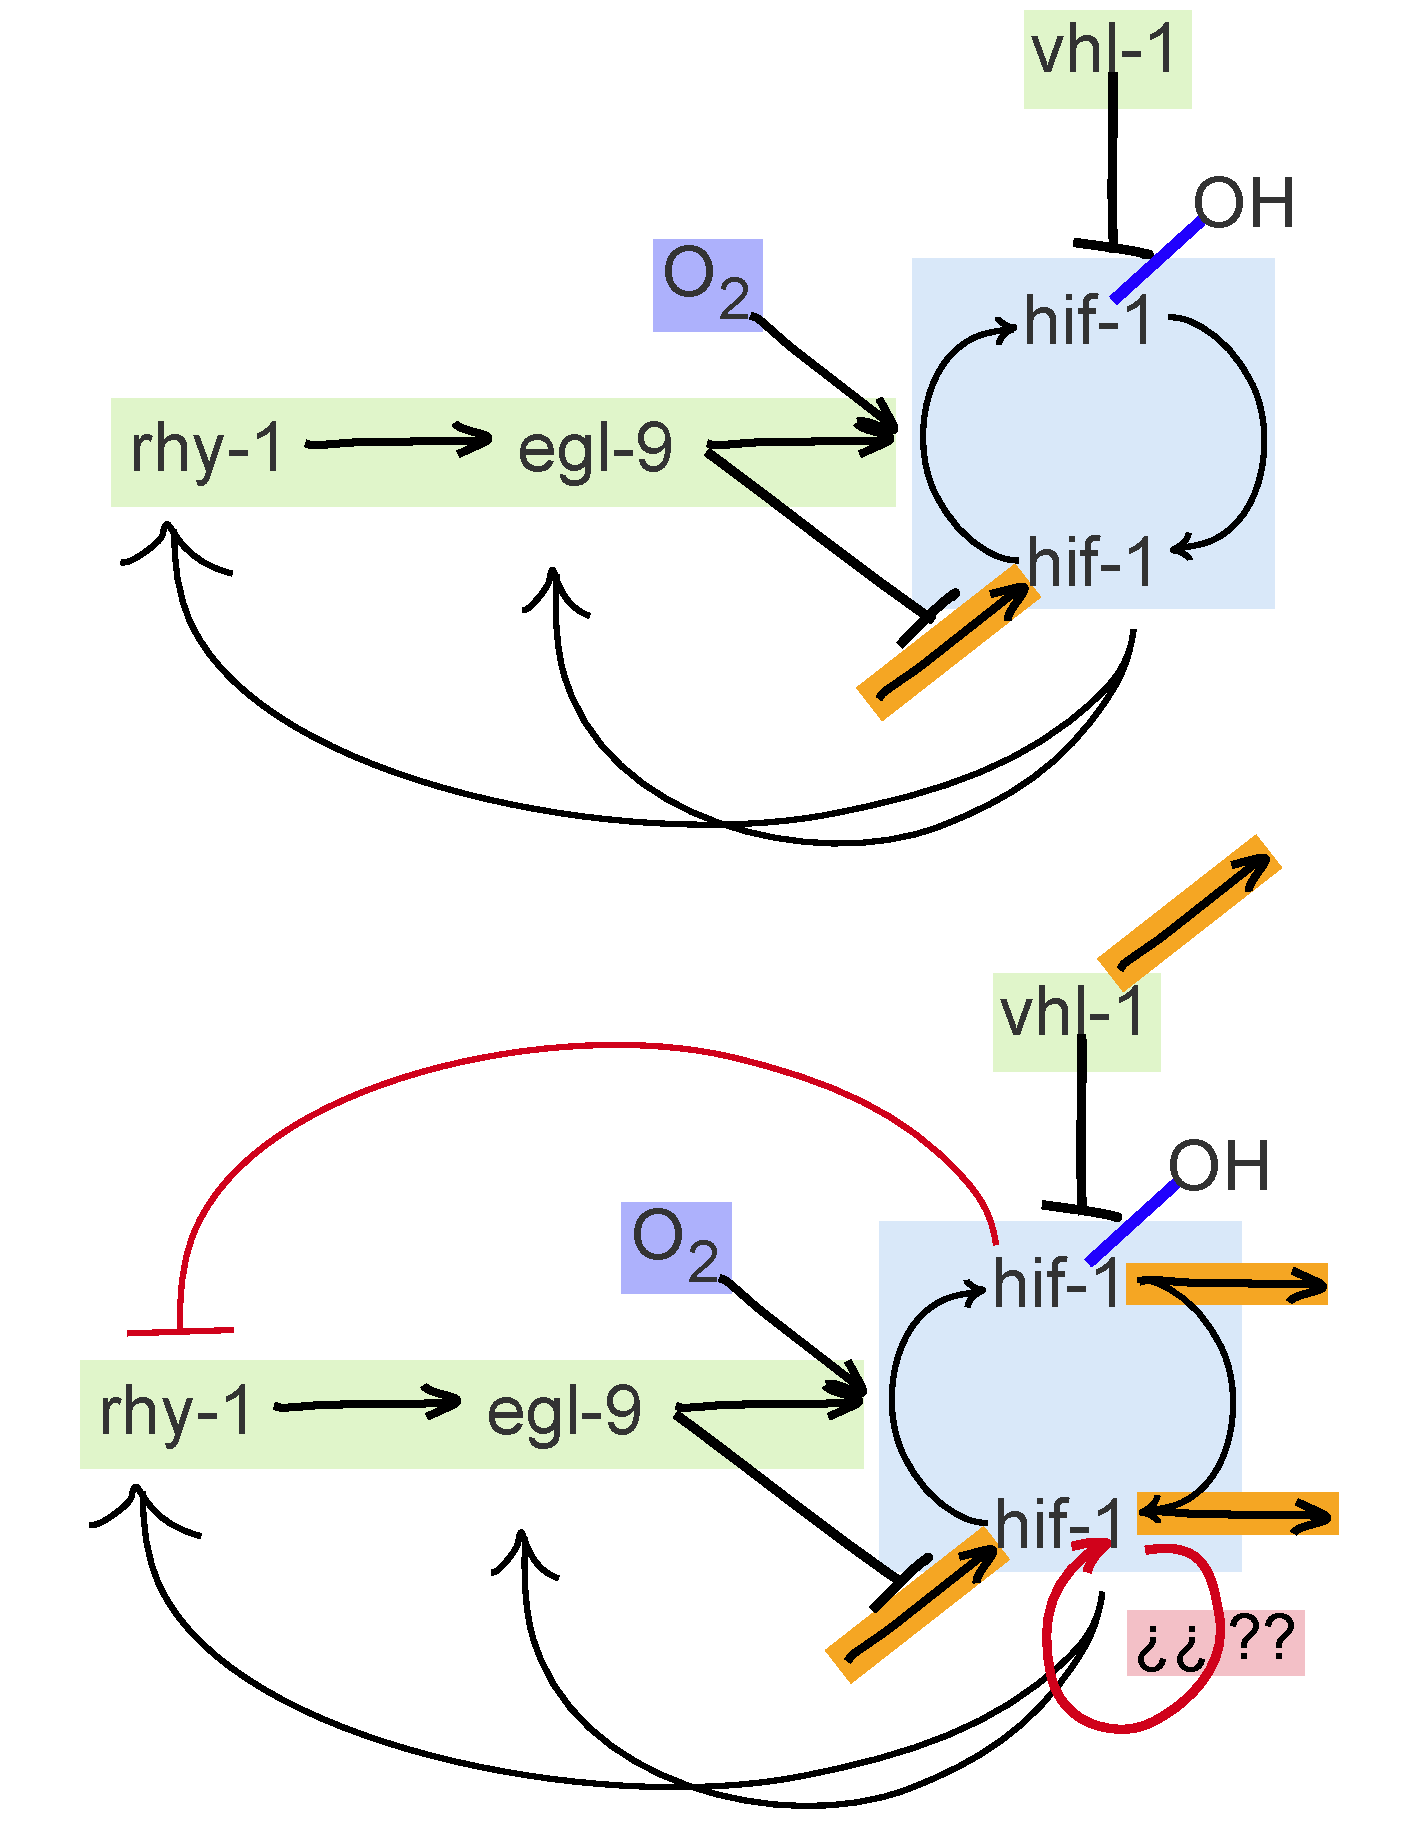
\includegraphics[width=\linewidth]{figs/new_model.pdf}
\caption{Top: Previous model. Bottom: Current model derived from RNA-seq data.}
\label{fig:newmodel}
\end{figure}

Previous work has established a circuit in which \rhy{} activates \egl{} in a linear pathway, and \egl{} inhibits \hif{} in an oxygen-dependent manner. Hydroxylated \hifp{} can then be degraded in a \vhl{}-dependent manner. There is also evidence that \egl{} and \rhy{} are in turn activated by \hif{}~\cite{Bishop2004,Powell-Coffman2010}.
Finally, there is evidence that although the interaction between \egl{} and \vhl{} is important for \hif{} repression, \egl{} can also act in a non-\vhl{} dependent manner (see Fig.~\ref{fig:newmodel} top).

From our data, we were able to impute the positive regulatory relationship between \egl{} and \rhy{}. We would not have been able to infer the order of the regulation without additional information. Using clustering as a proxy for phenotype, we were able to infer the relationship between \egl{} and \hif{}. We were also able to infer a positive (linear or AND) relationship between \egl{} and \vhl{} using clustering. Alternatively, we gained the same information by performing \emph{in silico} qPCR on the genes under study. \emph{In silico} qPCR also revealed that \hif{} has two states with different activities: Non-hydroxylated \hifp{} increases levels of \rhy{}, and hydroxylated \hifp{} inhibits \rhy{} and possibly \egl{} as well, although the double mutant did not recapitulate that interaction. We also revealed that \hif{} is an autoregulator.

These discoveries are consistent with a homeostatic circuit. By autoregulating itself, \hif{} can mantain appropriate protein levels both in normoxic and hypoxic conditions. Inhibition of \rhy{}, and possibly of \egl{}, ensures that an appropriate equilibrium is maintained between hydroxylated and non-hydroxylated protein, which may have functional consequences for the cell if both forms are active.

In addition to these biological findings, our dataset allows us to generate predictions of genes that may be under direct \hif{} regulation. Assuming that non-hydroxylated \hifp{} has different activities from hydroxylated \hifp{}, we identified 5 genes that are candidates for activation by hydroxylated \hifp{}. These genes have been implicated in the \cel{} immune response, or have behavioural phenotypes, underscoring the importance of \hif{} in neurobiology and immunology~\cite{Gray2004,Cheung2005,Chang2008,Ma2013}.
We have shown that transcriptomes contain sufficient information to be used as semi-quantitative phenotypes in metazoans. These phenotypes can be interpreted globally via correlation tests, clustering or other probabilistic methods; alternatively, they can be used to query single reporter genes in a manner similar to qPCR today. Transcriptomic phenotypes have distinct advantages over physical traits.
Firstly, due to their increased complexity, the genotype-phenotype mapping degeneracy ought to be greatly reduced, which facilitates predictions of genetic interaction. Secondly, genes that result in subtle or no visible traits when mutated may have strong (detectable), reproducible phenotypes at the transcriptomic level, which would make the study of small-effect genes significantly easier.

RNA-seq and microarray datasets have been used previously by bioinformaticians to generate high-throughput predictions of genetic interactions and consortiums such as the The Cancer Genome Atlas have sequenced RNA from many different cancers in the hope of identifying clinically or biologically relevant interactions~\cite{}. By correlating many different datasets in many different conditions, it is possible in theory to predict genetic interaction. Our approach differs from these high-throughput methods in that we are not attempting to generate large scale networks. Rather, the strength in our analysis derives from our experimental design, which allows us to ask and answer a large number of questions about the functional interactions between genes.
As a by-product, we are also able to identify genes related to the core circuit studied in question, but our main goal is not to generate databases or predict large numbers of interactions between a large number of genes. We have shown that transcriptomic phenotypes can capture distinct interaction modes in a single experiment, making it possible to infer complex regulatory relationships between genes. By measuring these transcriptomes under a rigorous experimental design, it is possible to identify many relationships simultaneously. With the advent of fast pseudo-alignment tools and ever cheaper sequencing techniques, biologists should consider using global transcriptomes as a tool beyond hypothesis generation or target acquisition.


\matmethods{
\label{methods}
\subsection*{RNA-seq}
Tagmentation etc

We used Kallisto to perform pseudo-read alignment and performed differential analysis using Sleuth. We fit a generalized linear model for a transcript $t$ in sample $i$:
\begin{equation}
  y_{t,i} = \beta_{t, 0} + \beta_{t, genotype}\cdot{}X_{t, i} + \beta_{t, batch}\cdot{}Y_{t, i} + \epsilon_{t, i}
\end{equation}

where $y_{t, i}$ are the logarithm transformed counts; $\beta_{t, genotype}$ and $\beta_{t, batch}$ are parameters of the model, and which can be interpreted as biased estimators of the log-fold change; $X_{t, i}, Y_{t, i}$ are indicator variables describing the conditions of the sample; and $\epsilon_{t, i}$ is the noise associated with a particular measurement.

\subsection*{Genetic Analysis}
Genetic analysis of the processed data was performed in Python 3.5. Our scripts made extensive use of the Pandas, Matplotlib, Scipy, Seaborn, Sklearn, Networkx, Bokeh, PyMC3, and TEA libraries~\cite{Team2014,McKinney2011,Oliphant2007,Pedregosa2012,Salvatier2015,VanDerWalt2011,Developers,Angeles-Albores2016,Waskom}.
Our analysis is available in a Jupyter Notebook\cite{Perez2007}. All code and required data (except the raw reads) are available at \url{https://github.com/WormLabCaltech/mprsq} along with version-control information. Our Jupyter Notebook and interactive graphs for this project can be found at \url{https://wormlabcaltech.github.io/mprsq/}. Raw reads were deposited at XXXXXXXXXXX.
}

\showmatmethods{}% Display the Materials and Methods section

\acknow{This article was written with support of the Howard Hughes Medical Institute.}

\showacknow{} % Display the acknowledgments section

% \pnasbreak splits and balances the columns before the references.
% If you see unexpected formatting errors, try commenting out this line
% as it can run into problems with floats and footnotes on the final page.
% \pnasbreak{}

% Bibliography
\bibliography{citations}

\end{document}
